\subsection*{Geo-Informations-Grundlagen}
Jeder Punkt auf der Erdkugel wird eindeutig durch die Kombination eines Breiten- und eines Längengrades definiert.
Breitengrade (Latitudes) liegen stets im Bereich von -90° (Süden) bis 90° (Norden). 0° beschreibt den Äquator.
Längengrade (Longitudes) werden von -180° (westlich) bis 180° (östlich) angegeben. Bei 0° befindet sich der Nullmeridian (Prime Meridian), welcher durch Greenwich (GB) verläuft.
Hierbei ergibt sich ein wesentliches mathematisches Problem.
Da -180° und +180° aufeinanderliegen, ist die rein mathematische Differenz zweier unmittelbar um diesen Meridian gelegenen Punkte größer als jede andere Differenz zweier Punkte.
Ein weiteres Problem ist die Uneinigkeit verschiedener Spezifikationen und Normen über die Reihenfolge der beiden Werte.
In diesem Projekt wird stets mit <longitude, latitude> gearbeitet.

\begin{figure}[h]
    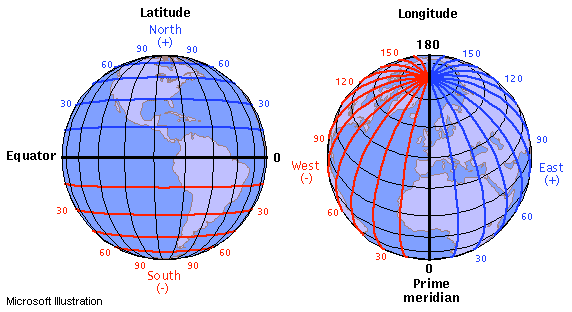
\includegraphics[width=\columnwidth]{images/lat-lon-world}
    \captionof{figure}{Latitude - Longitude}
\end{figure}

Für die Erfassung von Höhendaten gab es in der Vergangenheit verschiedene Projekte und Techniken.
Darunter fallen beispielsweise Lidar, Radar und Stereo-Photogrammetrie. Die so ermittelten Datensätze werden wiederum von verschiedenen Anbietern zur Verfügung gestellt.

Das vorgestellte Routingsystem unterstützt dabei wahlweise Open-Elevation oder OpenTopodata.
Mit einer geplanten Flughöhe von 150 m über dem Boden wird die Wahrscheinlichkeit einer Kollision mit menschengemachten Bauten zwar drastisch reduziert, jedoch gibt es einige Ausnahmen, etwa den Berliner Fernsehturm mit einer Höhe von über 350 m. Dies ist beim Einsatz in neuen Regionen zu beachten und zu planen. Um betreffende Bauwerke können manuell Sperrzonen eingerichtet werden. Trotzdem sollte die Flugsteuerung mit Kamera, Bilderkennung und einem Ausweichmechanismus gekoppelt sein.
Sogenannte Sperrzonen, welche aus sicherheitstechnischen Gründen nicht überflogen werden dürfen, da sie beispielsweise von militärischer Relevanz oder für den Regelflugbetrieb reserviert sind, werden über die Schnittstelle openAIP bezogen.